% ****** Start of file apssamp.tex ******
%
%   This file is part of the APS files in the REVTeX 4.1 distribution.
%   Version 4.1r of REVTeX, August 2010
%
%   Copyright (c) 2009, 2010 The American Physical Society.
%
%   See the REVTeX 4 README file for restrictions and more information.
%
% TeX'ing this file requires that you have AMS-LaTeX 2.0 installed
% as well as the rest of the prerequisites for REVTeX 4.1
%
% See the REVTeX 4 README file
% It also requires running BibTeX. The commands are as follows:
%
%  1)  latex apssamp.tex
%  2)  bibtex apssamp
%  3)  latex apssamp.tex
%  4)  latex apssamp.tex
%
\documentclass[%
 reprint,	
%superscriptaddress,
%groupedaddress,
%unsortedaddress,
%runinaddress,
%frontmatterverbose, 
%preprint,
showpacs,
% preprintnumbers,
%nofootinbib,
%nobibnotes,
%bibnotes,
 amsmath,amssymb,
 aps,
 prc,
%prb,
%rmp,
%prstab,
%prstper,
%floatfix,
]{revtex4-1}

\usepackage{graphicx}% Include figure files
\usepackage{dcolumn}% Align table columns on decimal point
\usepackage{bm}% bold math
\usepackage{url}
\usepackage{lipsum}
\usepackage{color}
\usepackage{hyperref}% add hypertext capabilities
\usepackage[mathlines]{lineno}% Enable numbering of text and display math
\usepackage{upgreek}
\usepackage{biolinum}
\linenumbers\relax % Commence numbering lines

%\usepackage[showframe,%Uncomment any one of the following lines to test 
%%scale=0.7, marginratio={1:1, 2:3}, ignoreall,% default settings
%%text={7in,10in},centering,
%%margin=1.5in,
%%total={6.5in,8.75in}, top=1.2in, left=0.9in, includefoot,
%%height=10in,a5paper,hmargin={3cm,0.8in},
%]{geometry}

% \setcounter{secnumdepth}{5}
\begin{document}

\preprint{APS/123-QED}

\title{Measurement of $\phi(1020)$-meson and $\Xi^{-}$ hyperon Production in Au+Au Collisions at ${\sqrt{s_{\rm NN}} = \rm{3\,GeV}}$}% Force line breaks with \\
%\thanks{A footnote to the article title}%

% \author{Ann Author}
% \altaffiliation[Also at ]{Physics Department, XYZ University.}%Lines break automatically or can be forced with \\
% \author{Second Author}%
% \email{Second.Author@institution.edu}
% \affiliation{% Authors' institution and/or address\\ This line break forced with \textbackslash\textbackslash
% }%

\collaboration{STAR Collaboration}
\noaffiliation

\date{\today}% It is always \today, today,
             %  but any date may be explicitly specified

\begin{abstract}


We report on the first measurement of $\phi$-meson and $\Xi^{-}$ hyperon production as well as the $\phi/K^-$ and $\phi/\Xi^-$ ratio in Au+Au collisions at ${\sqrt{s_{\rm NN}} = \rm{3\,GeV}}$ with the STAR experiment under its fixed target configuration at RHIC. $\phi$-mesons and $\Xi^{-}$ hyperons are measured through their hadronic decay channels, $\phi\rightarrow K^+K^-$ and $\Xi^-\rightarrow \Lambda\pi^-$. The transverse momentum ($p_T$) spectra of $K^-$, $\phi$ and $\Xi^{-}$ are presented in different centrality and rapidity intervals. The total production yields and the ratios within a $4\pi$ acceptance window are calculated and compared to thermal model predictions. The grand canonical ensemble (GCE) calculation shows a clear discrepancy from our measurement. Our data favors the canonical ensemble (CE) model with a strangeness correlation length of $r_c   \sim 3.2\rm{fm}$ in 0--10\% central Au+Au collisions at ${\sqrt{s_{\rm NN}} = \rm{3\,GeV}}$.


%\begin{description}
%\item[Usage]
%Secondary publications and information retrieval purposes.
%\item[PACS numbers]
%May be entered using the \verb+\pacs{#1}+ command.
%\item[Structure]
%You may use the \texttt{description} environment to structure your abstract; use the optional argument of the \verb+\item+ command to give the category of each item. 
%\end{description}
\end{abstract}

\pacs{25.75.-q, 25.75.Cj}% PACS, the Physics and Astronomy
                             % Classification Scheme.
%\keywords{Suggested keywords}%Use showkeys class option if keyword
                              %display desired
\maketitle

% Chapter one
% \section{Introduction}
% \label{introduction}

Relativistic heavy ion physics is aimed at the detailed investigation of phase structures of strongly interacting matter, governed by Quantum Chromodynamics (QCD), under conditions of extremely high temperature and density~\cite{akiba2015hot,StarWhitePaper}. Particle production has been studied to investigate the properties of the produced QCD matter in heavy ion collisions. 
Strange quark mass % provide a unique method to study the hot QCD medium in heavy-ion collisions since 
%because that their mass 
is comparable to the QCD scale 
%as well as to 
and
the temperature of the produced medium~\cite{Rafelski:1982pu,Koch:1986ud}, therefore strange quark dynamics plays an important role in understanding the QCD Equation-of-State, particularly in the high density region~\cite{KO_sQM17,Danielewicz1592,Tetyana_ICNN,KO.PhysRevLett.55.2661,HADES.Ks2019457,CASSING.openCharm.2001753}. 

Statistical thermal models have often been used to characterize the thermal properties of the produced media~\cite{BraunMunzinger:2003zd,Redlich_CE}. In these models, Grand Canonical Ensemble (GCE) and Canonical Ensemble (CE) statistical descriptions can be applied to conserved electric charge, baryon number, and strangeness number in order to compute the final state particle yields. Both GCE and CE models are able to describe various particle yields including strange particles produced in heavy-ion collisions at RHIC and the LHC at center-of-mass energy ($\sqrt{s_{\rm NN}}$) greater than 7.7\,GeV. It has been argued that at lower energies, strangeness number needs to be conserved on an event-by-event basis described by the CE, which leads to a reduction in the yields of hadrons with non-zero strangeness number (``Conanical Suppression")~\cite{Redlich:2001kb}.

The $\phi(1020)$ meson is the lightest bound state of $s\bar{s}$ with zero net strangeness number (S=0). %$\phi$ meson production in elementary collisions is suppressed compared to other strange hadrons due to the QCD Okubo-Zweig-Iizuka rule. 
In the GCE model, the $\phi/K^-$ ratio is expected to fall off when the collision energy decreases while in the CE model, $\phi$ meson production is not affected by the event-by-event strangeness number conservation, unlike other strange hadrons ($K^-$, $\Xi^-$ etc.). Therefore, the $\phi/K^-$ ratio is expected to increase with decreasing collision energy in models using the CE treatment for strangeness. The canonical suppression power for $\Xi^-$ is even larger compare to $K^-$. The $\phi/K^-$ and $\phi/\Xi^-$ ratios offer a unique test to scrutinize thermodynamic properties of strange quarks in the hot and dense QCD environment.

% ?? do we need this paragraph?
In heavy ion collisions, the near/sub-threshold production of multi-strange hadrons can achieve by accumulating multiple collisions involve nucleons, produced particles and short-living resonances. The particle production in heavy ion collisions below its free nucleon-nucleon (NN) threshold ($\sqrt{s_{\rm NN}}$ $\sim$2.89\,GeV for $\phi$ and $\sim$3.25\,GeV for $\Xi^-$) is expected to be sensitive to the stiffness of nuclear equation of state at high density, similar to single-strange hadrons~\cite{KO.PhysRevLett.55.2661,FUCHS20061_kaons}. The near/sub-threshold production further provides the possibility to find the signals of the missing baryon resonance and the decay channels that are not yet observed in experiments~\cite{Steinheimer_2015_UrQMD,KO_sQM17}. 

Measurements from the AGS, SPS, RHIC and LHC show that the $\phi/K^-$ ratio in heavy-ion collisions stays remarkably flat ($\sim$0.15) at collision energies $\sqrt{s_{\rm NN}}\,>\,$5\,GeV. Recent measurements of the $\phi/K^-$ ratio in heavy-ion collisions at collision energies below the $\phi$ free NN-threshold from HADES and FOPI show a hint of relative enhancement compared to those from high energies at RHIC and the LHC~\cite{E917_phi,NA49_phi,FOPI_phi_AlAl,FOPI_phi_NiNi,HADES_phi_ArKCl,HADES_phi_AuAu}, indicative of the applicability of the CE description for strangeness production at these energies. %In the CE model, a correlation length, $r_c$, is often used to characterize the volume size to account for local strangeness conservation, which remains largely uncertain with the existing measurements.
The RHIC Beam Energy Scan phase-II program, including both collider and fixed target setups with the STAR experiment, covers a center-of-mass energy range of 3.0--19.6\,GeV. This offers us a great opportunity to conduct precise measurement of the energy dependence of the $\phi/K^-$ and $\phi/\Xi^-$ ratio at low collision energies, which is crucial to understand the strangeness dynamics as well as the medium properties at high baryon density regions in QCD.


The dataset used in this analysis consists of Au+Au collisions at ${\sqrt{s_{\rm NN}} = \rm{3\,GeV}}$ collected by the STAR experiment operated under the fixed target (FXT) setup in the 2018 RHIC run. %For the FXT configuration used here, 
A single beam was provided by RHIC with total energy equal to 3.85 GeV and incident on a gold target of thickness 0.25 mm, corresponding to a 1\% interaction probability.
%to minimize the pileup and energy loss effect in target.
The target is installed inside the vacuum pipe, 2\,cm below the center of the beam axis, and located 200\,cm to the west of the center of the STAR detector. The main detectors used are the Time Projection Chamber (TPC)~\cite{TPC}, the Time of Flight (TOF) detector~\cite{TOF} and the Beam-Beam Counter (BBC). The trigger system is provide by the BBC detector, while tracking and particle identification are done using the TPC and TOF. Events are selected with the offline reconstructed collision vertex within 1.5\,cm of the target centers along the beam direction. Approximately 2.6$\times 10^{8}$ minimum bias (MB) triggered events pass the selection criteria and are used in this analysis. 

The centrality class is selected using measured charged particle multiplicity within the TPC acceptance. 
A Monte Carlo Glauber model in conjunction with a negative binomial distribution used to model particle production is optimized in order to best match the data and determine the centrality class. Due to the trigger inefficiency in the low multiplicity region (corresponding to most peripheral collision), and finite contribution to our interested signals, we only report the results from the 0--60\% centrality class in this paper.

The $\phi$-mesons are reconstructed via the hadronic decay channel $\phi\rightarrow K^+K^-$ with a branching ratio ($B.R.$) of 49.2\%, while the $\Xi^{-}$ hyperons via the $\Xi^-\rightarrow \Lambda\pi^-\rightarrow p\pi^-\pi^-$ channel with a BR of 63.8\%~\cite{pdg}. $\Xi^-$ reconstruction are performed using the KF Particle Finder package based on the Kalman Filter method
%initially developed from the CBM and ALICE experiments
~\cite{Kisel:2018nvd}. The charged tracks are reconstructed with the TPC in a 0.5-T uniform magnetic field. The TPC tracks are required to contain at least 20 TPC hits (out a maximum of 45) to ensure a good tracking and avoid track splitting (15 TPC hits required for $\Xi^{-}$ to enlarge statistics of signal candidates). The charged tracks are identified via a combination of the ionization energy loss %($dE/dx$) 
measurement with the TPC and the time-of-flight %($tof$) 
measurement with the TOF.
%, which have been extensively used in many prior STAR analyses. 
Due to the charge asymmetry for the particle yields at ${\sqrt{s_{\rm NN}} = \rm{3\,GeV}}$, a smaller yield for $K^-$ means a relative higher contaminations, thus a strict PID requiring both TPC and TOF are implemented~\cite{Xu:2008th,Shao:2005iu}. Both the TPC and TOF detectors have full azimuthal coverage within a pseudo-rapidity range of 0$<$\,$\eta$\,$<$\,1.88 for the TPC and 0$<$\,$\eta$\,$<$\,1.5 for the TOF in FXT mode~\cite{TPC,TOF}.



\begin{figure}
\centering
\hspace*{-4mm}
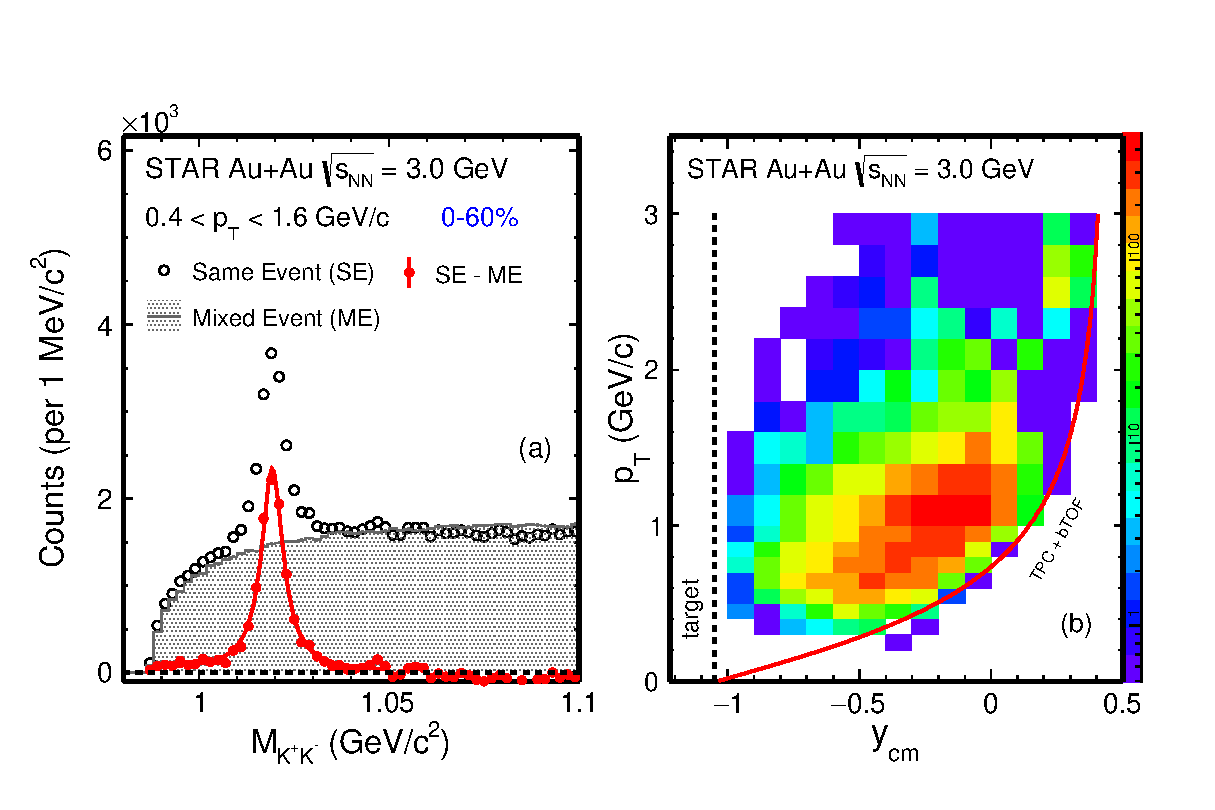
\includegraphics[width=0.48\textwidth]{fig/fig1_signal.eps}
  \caption{Invariant mass distributions of $K^+K^-$ (a) and $\Lambda(p\pi^-)\pi^-$ (b) in the $p_T$ region of 0.4--1.6\,GeV/$c$ in 0--60\% and 0.5--2.0\,GeV/$c$ in 0--40\% central Au+Au collisions at ${\sqrt{s_{\rm NN}} = \rm{3\,GeV}}$, respectively. Black open circles represent the same-event unlike-sign distribution. The grey shaded histogram represents the normalized mixed-event (rotational) for $\Xi^-$) unlike-sign distribution that is used to estimate the combinatorial background. The red solid circles depict the $\phi$-meson (a) and $\Xi^-$ (b) signals obtained by subtracting the combinatorial background from the same-event distribution. Reconstructed $\phi$-meson (c) and $\Xi^-$-hyperon (d) acceptance $p_T$ vs. rapidity in the center-of-mass frame ($y_{\rm cm}$) in Au+Au collisions at ${\sqrt{s_{\rm NN}} = \rm{3\,GeV}}$. The dotted line at $y_{\rm cm}$ indicates the target rapidity location and the solid red line indicate the acceptance edge for charged kaon tracks selected by TPC + barrel TOF (bTOF).}
\label{fig:phiSignal} 
\end{figure}


Figure~\ref{fig:phiSignal} (a) shows the invariant mass distribution of $K^+K^-$ pairs in the $p_{T}$ region of 0.4--1.6 GeV/$c$ for 0--60\% central collisions. The combinatorial background is estimated with the mixed-event (ME) technique in which $K^+$ and $K^-$ from different events of similar characteristics (centrality, event plane angle) are paired. The mixed-event spectra are normalized to the same-event (SE) distributions in the mass range of 1.04--1.08\,GeV/$c^2$. After the subtraction of the combinatorial background, the remainder distribution is shown as red solid circles. The remainder $K^+K^-$ invariant mass distributions are fit with a Breit-Wigner for the signal plus a linear function represent the remaining correlated background. The $\phi$-meson raw yields are extracted from the Breit-Wigner function fit within the corresponding mass windows. The extracted $\phi$ signal shape is consistent with its intrinsic properties convoluted with the detector smearing effect due to finite momentum resolution.
Figure~\ref{fig:phiSignal} (b) shows the invariant mass distribution of $\Lambda(p\pi^-)\pi^-$ in the $p_{T}$ region of 0.5--2.0 GeV/$c$ for 0--40\% central collisions. The combinatorial background is estimated with the rotate-event (RE) method in which a daughter track of $\Xi^-$ is rotated by a random angle between 150 to 210 degrees in transverse plane. The rotate-event spectra are normalized to the same-event (SE) distributions in the mass range of 1.30--1.31 and 1.34--1.35\,GeV/$c^2$. As the combinatorial background subtracted, $\Lambda\pi^-$ invariant mass distributions are fit with a Gaussian for the signal plus a linear function for the remaining correlated background. The $\Xi^-$ raw yields are obtained via histogram bin counting from the invariant mass distributions with all background subtracted within mass windows of 3$\sigma_{mass}$. The reconstructed $\phi$-meson and $\Xi^-$ acceptances ($p_T$ vs. $y_{cm}$) in the collision center-of-mass frame are shown in Fig.~\ref{fig:phiSignal} (c) and (d), respectively.
The target is located around $y_{cm}$ = -1.05, using the convention where the beam travels in the positive direction. The red curve represents the TPC and TOF acceptance edge. The reconstructed $\phi$-mesons and $\Xi$-hyperons in this analysis cover the range from the target to mid-rapidity.


The reconstructed $K^-$, $\phi$-meson, and $\Xi^-$ raw yields are calculated in each centrality and $p_{T}$ bin within each rapidity slice. 
%The corrected $\phi$-meson, $K^-$ and $\Xi^-$ production invariant yields can be calculated 
%using the following formula:
%\begin{equation*}
%  \begin{aligned}
% \frac{d^2N}{2\pi p_{T}dp_{T}dy} = \frac{1}{\rm B.R.} \times \frac{N^{\rm raw}}{N_{\rm evt} 2\pi p_{T}\Delta p_{T}\Delta y} \times \frac{1}{\varepsilon_{\rm TPC}\times\varepsilon_{\rm PID}\times\varepsilon_{\rm TOF}},
%  \end{aligned}
%\label{equ:invariantyield}
%\end{equation*}
%where B.R. is the corresponding decay branching ratio, $N^{\rm raw}$ is the reconstructed raw count, and $N_{\rm evt}$ is the total numbers of events in the corresponding centrality bins. 
The raw yields are corrected for the TPC acceptance and tracking efficiency, %$\varepsilon_{\rm TPC}$, 
the particle identification efficiency, %$\varepsilon_{\rm PID}$ 
and the TOF matching and PID efficiency. The final average reconstruction efficiency for 0.30 for $K^-$, $\phi$-meson is about 0.04 and 0.02 for $\Xi^-$.

\begin{figure}
\centering
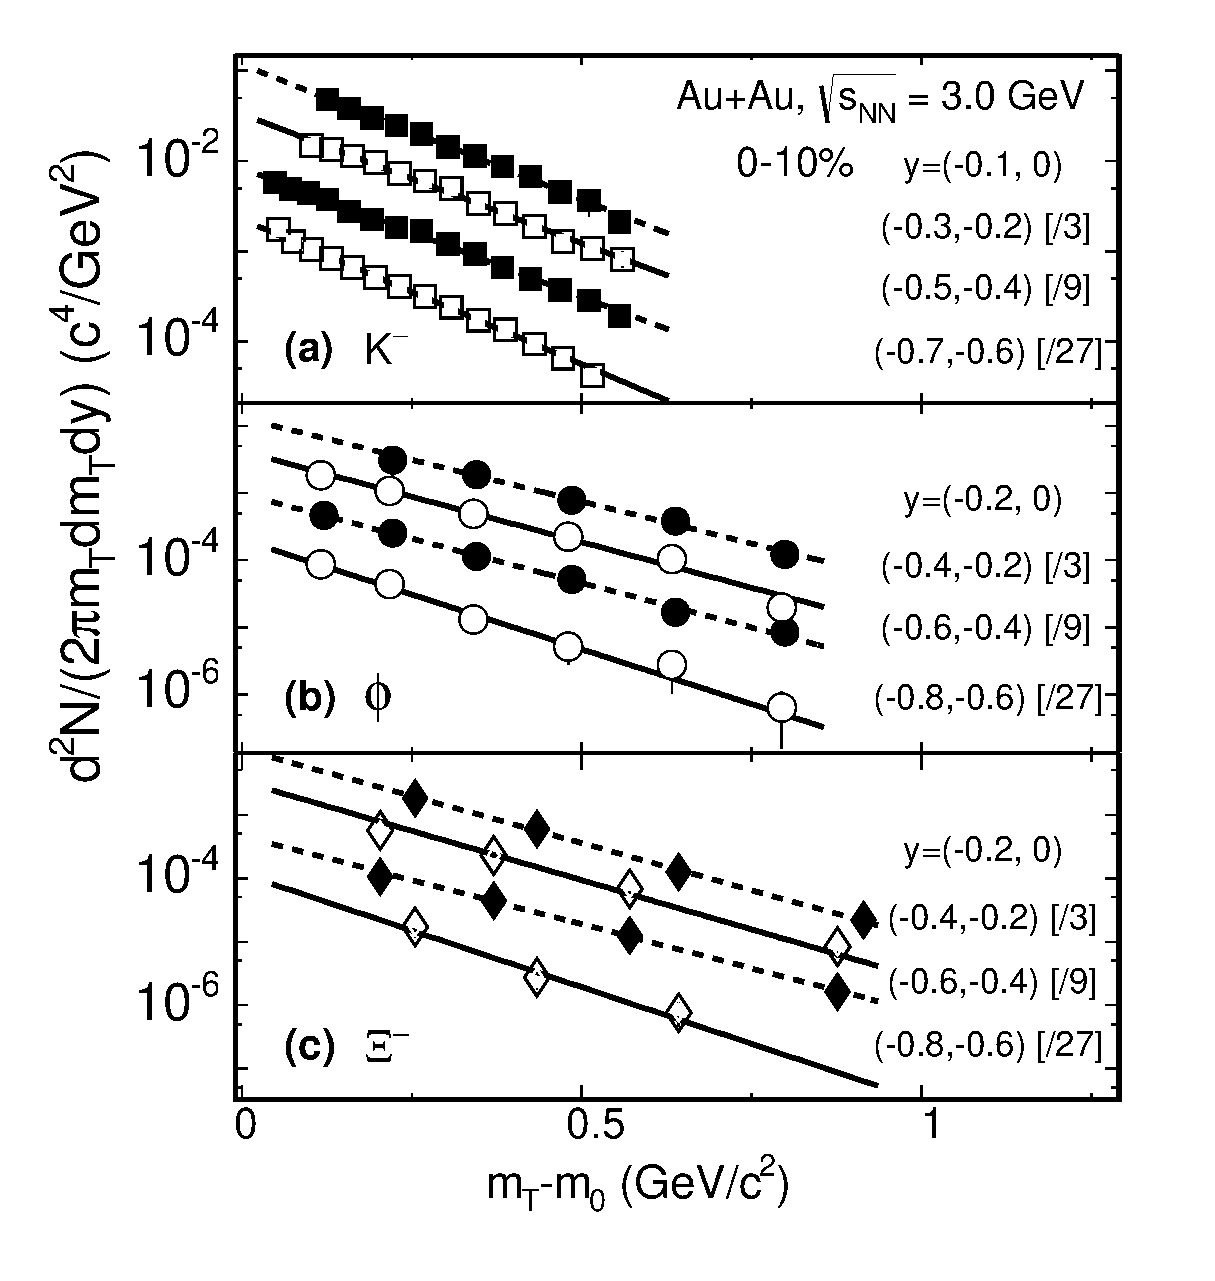
\includegraphics[width=0.41\textwidth]{fig/fig2_h_mT_spectra_phiMeson.eps}
  \caption{ $K^-$, $\phi$-meson and $\Xi^-$ invariant yields as a function of transverse mass kinetic energy ($m_T-m_0$) for various rapidity regions in 0--10\% central Au+Au collisions at ${\sqrt{s_{\rm NN}} = \rm{3\,GeV}}$. Solid and dashed black lines depict exponential function fits to the measured data points.}
\label{fig:phimTSpectra} 
\end{figure}

The systematic uncertainty of the raw yield extraction is estimated by changing the raw yield counting method from the fit to histogram bin counting or changing the fitting ranges. The maximum difference between these scenarios is then converted to a standard deviation and added to the systematic uncertainties. The contribution varies by $p_T$, rapidity, and centrality %since the statistics are correlated, but 
and the overall contribution is less than 5\% for the total cross section. The systematic uncertainty in the TPC acceptance and efficiency correction $\varepsilon_{\rm TPC}$ is estimated %via the standard procedure in STAR by %comparing the TPC track distributions between real data and the embedding data, then 
by varying the cuts on track selection criteria and topological variables (for $\Xi^-$ only). %such as the number of fit points and DCA used for tracking. 
%After correcting for the corresponding efficiency for each scenario, the difference is added to the systematic uncertainties. The acceptance and efficiency contributions for $\Xi^-$ is correlated to the topological variables used for reconstruction. 
The contribution to the total yield is about 4-5\% for $K^-$, 13-16\% for $\phi$ and 6-10\% for $\Xi^-$. This leads to a 10-13\% (12-18\%) uncertainty in the measured $\phi/K^-$ ($\phi/\Xi^-$) ratio. 
The uncertainty of the PID efficiency correction is estimated in a similar way by varying the PID selection cuts and the contribution is less than 3\% to the total yield.
%such as the TPC $n\sigma_{K}$ and TOF $1/\beta$ and then propagating these changes to the final corrected yield. This source contributes 2-3\% to the total systematic uncertainty.  
%a combined contribution is about 6-10\% in the reported 2 centrality bins and results in a 12-18\% uncertainties in the measured $\phi/\Xi^-$ ratio. 
For the $p_T$ integrated yield, one important source of systematic uncertainty comes from the extrapolation to the full $p_T$ range due to the limited acceptance. This is estimated by choosing several different fitting functions %including Levy, Blast-Wave, $m_T$-exponential, $p_T$-exponential and $p_T$-Gaussian
~\cite{STAR_particleYield}. The maximum difference between these scenarios and the default one ($m_T$-exponential) is quoted as the systematic uncertainty from this source. This contribution is 5-7\% for $K^-$, 14-17\% for $\phi$ and 13-15\% for $\Xi^-$. 
%For each individual $\phi$-meson, $K^-$ and $\Xi^-$ measurement, some of the uncertainties are correlated or partially correlated (e.g. TPC and PID). To avoid the correlation in the ratio measurement, we vary the above cuts simultaneously for $\phi$, $K^-$ and $\Xi^-$, then quote the final ratio difference directly as the systematic uncertainties.


%\begin{table*}
%\centering{
%  \caption{$\phi$, $K^-$ and $\Xi^-$ integrated yield and $T_{\rm eff}$ as well as $\phi/K^-$ and $\phi/\Xi^-$ ratios for given centrality classes in Au+Au collisions at ${\sqrt{s_{\rm NN}} = \rm{3\,GeV}}$. The first given error corresponds to the statistical, the second to the systematic error.}
%\begin{tabular}{c|c|c|c|c|c} \hline \hline
%  Centrality & $\langle\phi\rangle$ $(10^{-3})$  & $\phi$ $T_{\rm eff}$ (MeV) & $\langle K^-\rangle$ $(10^{-2})$ & $K^-$ $T_{\rm eff}$ (MeV) & $\langle\phi\rangle/\langle K^-\rangle$   \\ \hline
%  ~~~0--10\%~~~   & ~~~$20.1\pm1.4\pm3.8$~~~  & ~~~$177\pm5\pm8$~~~  & ~~~$8.70\pm0.02\pm 0.53$~~~  & ~~~$158\pm3\pm3$~~~ & ~~~$0.231\pm0.016\pm0.042$~~~ \\
%  10--40\%  & $8.45\pm0.4\pm1.7$  & $159\pm4\pm5$   & $3.39\pm0.01\pm 0.20$  & $142\pm3\pm3$ & $0.249\pm0.011\pm0.046$ \\
%  40--60\%  & $2.60\pm0.2\pm0.5$  & $151\pm5\pm11$   & $0.79\pm0.01\pm 0.06$  & $115\pm4\pm4$ & $0.327\pm0.029\pm0.069$ \\ \hline
%\end{tabular}
%\begin{tabular}{c|c|c|c} \hline
%  Centrality & $\langle\Xi^-\rangle$ $(10^{-3})$  & $\Xi^-$ $T_{\rm eff}$ (MeV) & $\langle\phi\rangle/\langle \Xi^-\rangle$   \\ \hline
%  ~~~0--10\%~~~   & ~~~$13.87\pm0.76\pm2.36$~~~  & ~~~$156\pm3\pm24$~~~  & ~~~$1.45\pm0.13\pm0.34$~~~ \\
%  10--40\%  & $3.61\pm0.32\pm0.59$  & $146\pm4\pm17$ & $2.34\pm0.23\pm0.65$ \\ \hline \hline
%\end{tabular}
%\label{table:yieldTratio}
%}
%\end{table*}

\begin{table*}
\centering{
  \caption{$\phi$, $K^-$, $\Xi^-$ integrated yields and $\phi/K^-$ and $\phi/\Xi^-$ ratios for given centrality classes in Au+Au collisions at ${\sqrt{s_{\rm NN}} = \rm{3\,GeV}}$. The first given error corresponds to the statistical one, the second to the systematic error.}
\begin{tabular}{c|c|c|c|c|c} \hline \hline
  Centrality & $\langle\phi\rangle$ $(10^{-3})$  & $\langle K^-\rangle$ $(10^{-2})$ & $\langle\phi\rangle/\langle K^-\rangle$ & $\langle\Xi^-\rangle$ $(10^{-3})$ & $\langle\phi\rangle/\langle \Xi^-\rangle$  \\ \hline
  ~~~0--10\%~~~   & ~~$20.1\pm1.4\pm3.8$~~  & ~~$8.70\pm0.02\pm 0.53$~~  & ~~$0.231\pm0.016\pm0.042$~~ & ~~$13.9\pm0.8\pm2.4$~~ & ~~$1.45\pm0.13\pm0.34$~~ \\
  10--40\%  & $8.5\pm0.4\pm1.7$  & $3.39\pm0.01\pm 0.20$  & $0.249\pm0.011\pm0.046$ & $3.61\pm0.32\pm0.59$ & $2.34\pm0.23\pm0.65$ \\
  40--60\%  & $2.6\pm0.2\pm0.5$  & $0.79\pm0.01\pm 0.06$  & $0.327\pm0.029\pm0.069$ & --- & --- \\ \hline
\end{tabular}
\label{table:yieldTratio}
}
\end{table*}

\begin{figure}
\centering
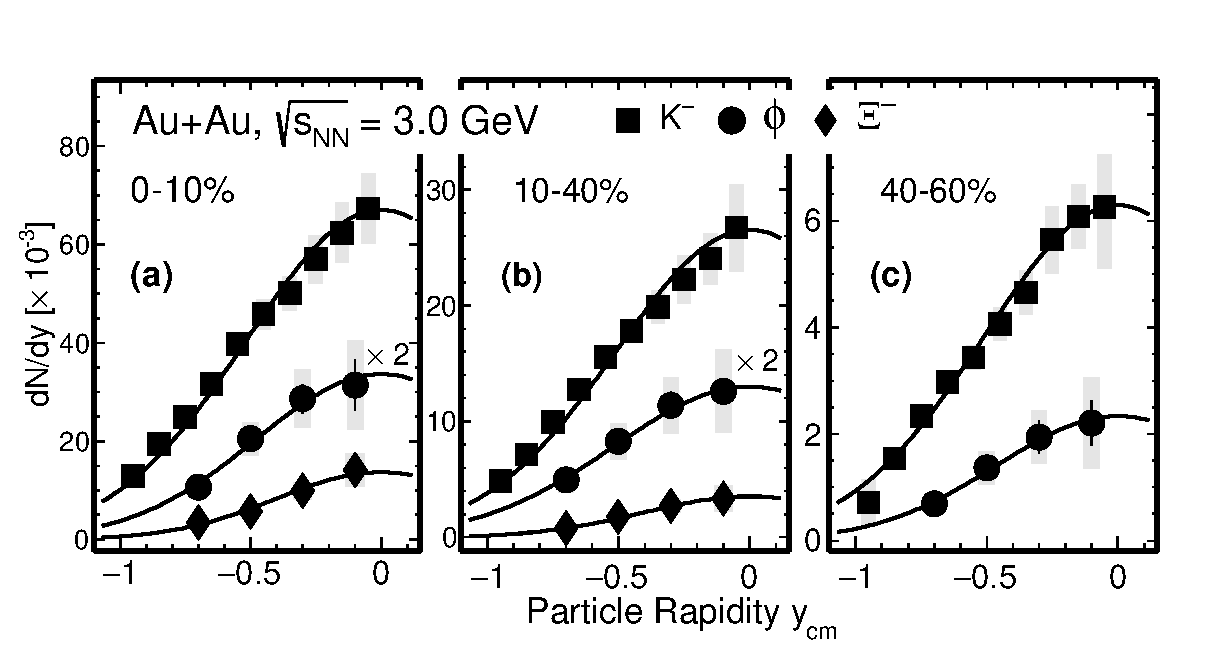
\includegraphics[width=0.48\textwidth]{fig/fig3_dndy.eps}
  \caption{ Rapidity density distributions of $K^-$ (squares), $\phi$-meson (circles) and $\Xi^-$ (diamonds) $p_T$-integrated yields $dN/dy$ in 0--10\% (a), 10--40\% (b) and 40--60\% central (c) Au+Au collisions at ${\sqrt{s_{\rm NN}} = \rm{3\,GeV}}$. %The full symbols show the measured data, while the open ones are data reflected with respect to $y=0$ in the center-of-mass frame. 
  Solid lines depict Gaussian function fits to the data points.}
\label{fig:phiYSpectra} 
\end{figure}

Figure~\ref{fig:phimTSpectra} shows the efficiency-corrected $\phi$-meson, $K^-$ and $\Xi^-$ invariant yields as a function of transverse mass kinetic energy ($m_T-m_0$) for various rapidity ranges in 0--10\% centrality Au+Au collisions at ${\sqrt{s_{\rm NN}} = \rm{3\,GeV}}$. %The $\phi$-meson, $K^-$ and $\Xi^-$ spectra in some rapidity intervals are scaled with arbitrary factors indicated in the figure for clarity. 
Dashed and solid lines depict fits to the spectra with the $m_T$-exponential function in order to extrapolate the unmeasured $p_T$ ranges. 
%The fitted inverse slope parameters indicate harder spectra for the $\phi$-mesons compared to the $K^-$ and $\Xi^-$ within uncertainties. The inverse slope parameters gradually decrease from mid-rapidity to forward/backward rapidity and follow the $T_{\rm eff}/\cosh(y)$ distribution well. The inverse slope parameter at $y=0$, $T_{\rm eff}$, is extracted to be $177\pm5_{stat}\pm8_{sys}$\,MeV for $\phi$ meson in 0--10\% central collisions. This agrees with the collision energy dependence trend from other experiments~\cite{HADES_phi_AuAu,FOPI_phi_NiNi,FOPI_phi_AlAl,HADES_phi_ArKCl,NA49_phi}.
%The rapidity density distributions are obtained for $\phi$, $K^-$ and $\Xi^-$ by integrating the measured data points in Fig.~\ref{fig:phimTSpectra} and using the exponential fits to extrapolate to the unmeasured region of phase space. 
The $p_T$ integrated rapidity distributions $dN/dy$ are displayed in Fig.~\ref{fig:phiYSpectra} for Au+Au collisions at ${\sqrt{s_{\rm NN}} = \rm{3\,GeV}}$ for three different centralities. %The full symbols show the measured data, while the open ones are data reflected with respect to $y=0$ in the center-of-mass frame. 
Solid lines depict Gaussian function fits to the data points with the centroid parameter fixed to zero. They are used to extrapolate to the unmeasured rapidity region in order to calculate the total multiplicities per triggered event for each particle.
%In the fitting procedure, the center of the Gaussian was fixed at zero to take into account the symmetry of the reaction. By integrating the measured rapidity and using the Gaussian fit to extrapolate, the multiplicities per triggered event of the $\phi$, $K^-$ and $\Xi^-$ are obtained.

The excitation function of $\phi/K^-$ and $\phi/\Xi^-$ ratios is presented in Fig.~\ref{fig:phi2Kratio} as a function of collision energy $\sqrt{s_{\rm NN}}$, including data from the AGS and SPS at higher energies and data from SIS at lower energies. The colored full symbols show our measurements in 0-10\% centrality bins in Au+Au collisions at ${\sqrt{s_{\rm NN}} = \rm{3\,GeV}}$. The measured $\phi$, $K^-$ and $\Xi^-$ yields in 4$\pi$ and the $\phi/K^-$, $\phi/\Xi^-$ ratios in different centrality bins are listed in Tab.~\ref{table:yieldTratio}. The $\phi/K^-$ ratio from this measurement is significantly ($5\sigma$) above the GCE prediction ($\sim$0), and slightly higher than the value ($\approx0.15$) at high energies for $\sqrt{s_{\rm NN}}\geqslant$ 5\,GeV~\cite{NA49_phi,NA49_piK,NA49_piK2,E917_phi,ALICE_phi_2p7TeV,STAR_phi_64a200GeV}. The measured data points follow the energy dependence trend, with the value gradually increasing with decreasing energy at low $\sqrt{s_{\rm NN}}$. %Our measured data points confirmed this enhancement observation which limited by the precision in the previous measurements. 
Though there is no clear difference in the $\phi/K^-$ ratio between the 0--10\% and 10--40\% central bins, the result in the most peripheral 40--60\% central bin shows a hint of a larger value. For comparison, a previous measurement in $p$+$p$ collisions at 2.7 GeV shows that $\phi/K^- = 1.04\pm0.23$ ~\cite{ANKE_phi}. 
%The measured data in mid-central 10-40\% collisions show a similar hint of larger value compare to most central 0-10\% collisions.

\begin{figure}
\centering
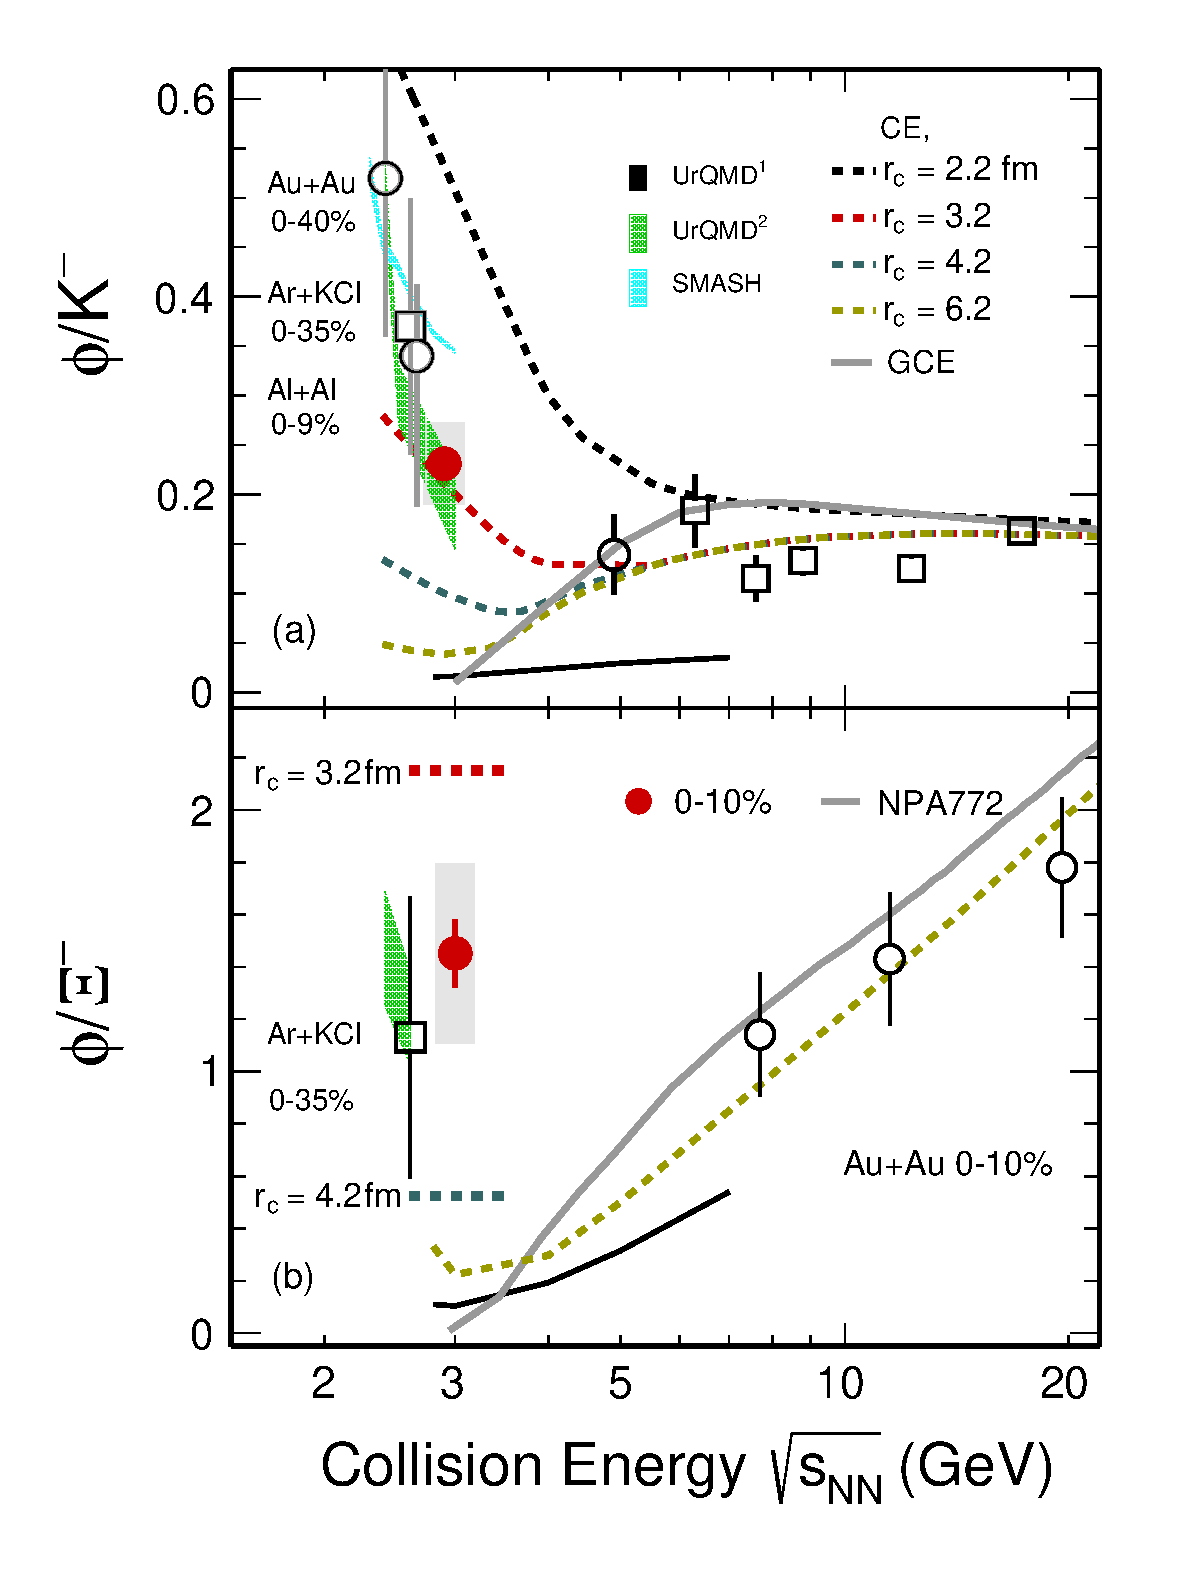
\includegraphics[width=0.42\textwidth]{fig/fig4_phi_over_kminus_zoomin.eps}
  \caption{ $\phi/K^-$ and $\phi/\Xi^-$ ratio as a function of collision energy $\sqrt{s_{\rm NN}}$. The full colored symbols show the measurements presented here in 0-10\% centrality bin, while markers in black or grey are used for data from various other energies and/or collision systems~\cite{E917_phi,NA49_phi,FOPI_phi_AlAl,FOPI_phi_NiNi,HADES_phi_ArKCl,HADES_phi_AuAu,Xi_ArKCl_HADES,star_bes_strangeness}. The grey solid line in (a) represents a thermal model calculation based on Grand Canonical Ensemble (GCE) while the dotted lines depict calculations based on Canonical Ensemble (CE) with different parameters of strangeness correlation radius ($r_c$)~\cite{Redlich_CE,Redlich_CE_private}, in (b) represents a thermal model calculation~\cite{ANDRONIC2006167_SHM}. The black, green and blue bands show transport model calculations from public version UrQMD~\cite{urQMD,UrQMD_2}, modified UrQMD~\cite{Steinheimer_2015_UrQMD} and SMASH~\cite{Elfner_SMASH}, respectively.}
\label{fig:phi2Kratio} 
\end{figure}


%Despite the different collision system and size including Au+Au, Ni+Ni, Ar+KCl and Al+Al, all of them observed substantially larger ratio in the low energy compared to high energies. 
Various curves in the Fig.~\ref{fig:phi2Kratio} (a) represent the predictions of $\phi/K^-$ from several model calculations. The Grand Canonical Ensemble (GCE) uses the chemical freeze-out parameters derived from the fits of experimental data at mid-rapidity with details in~\cite{ANDRONIC2006167_SHM}. The strangeness ($\mu_s$) is conserved on average in GCE, where the model does not contain a strangeness suppression factor which accounts for non-equilibrium in the strangeness sector. The model calculations are for midrapidity, while the experimental measurements are for total multiplicity, despite this, the model reproduces the AGS data well, while slightly deviating from the SPS measurements. It is clear that the model fails to describe the data at low energies, including our new measurements at ${\sqrt{s_{\rm NN}} = \rm{3\,GeV}}$, which may indicate the thermal particle phase-space at low energies is far from the GCE limit and the local treatment of strangeness conservation is crucial~\cite{BraunMunzinger:2003zd}. In the canonical approach, the correlation length, $r_c$, relates to a reduction of the particle production phase space inside which the production of the open strangeness is canonically conserved. There are 4 different $r_c$ calculations shown in Fig.~\ref{fig:phi2Kratio} (a). With a large $r_c$ = 6.2\,fm, the CE calculation gives a similar result as the GCE calculation. Assuming a linear interpolation with the $r_c$ calculations, and taking into account the statistics and systematic uncertainties of the measured data, %our result favors $r_c = 3.2_{-0.2}^{+0.2}$\,fm in 0--10\% central, $3.1_{-0.2}^{+0.2}$\,fm in 10--40\% centrality and $2.8_{-0.3}^{+0.2}$\,fm in 40--60\% central Au+Au collisions at ${\sqrt{s_{\rm NN}} = \rm{3\,GeV}}$.
our result favors $r_c \sim 3.2$\,fm in 0--10\% central, $\sim 3.1$\,fm in 10--40\% centrality and $\sim 2.8$\,fm in 40--60\% central Au+Au collisions at ${\sqrt{s_{\rm NN}} = \rm{3\,GeV}}$.
Note, the calculation using $r_c = 1.2$\,fm is consistent with the measured $\phi/K^-$ ratio in $p+p$ collisions at 2.7 GeV from ANKE~\cite{ANKE_phi,HADES_phi_ArKCl}. 

In Fig.~\ref{fig:phi2Kratio} (b), the $\phi/\Xi^-$ ratio from this measurement is larger than ($4\sigma$) the model calculation based on the GCE statistics including an additional fudge factor for strangeness canonical suppression with $V_C=1000$\,fm$^3$ ($r_c\sim6.2$\,fm). Dotted lines depict THERMUS calculations using strangeness CE with $r_c$ = 3.2, 4.2 and 6.2\,fm, respectively ($T_{ch}$ = 80\,MeV, $\mu_B$ = 720\,MeV, $\mu_S$ = 240\,MeV, $\mu_Q$ = 0, $\gamma_s = 1$ and $r$ = 6.2\,fm from the previous parameterization~\cite{CE_Cleymans}). The measured $\phi/\Xi^-$ ratio at 3\,GeV favors a $r_c$ parameter between 3.2 and 4.2\,fm. 
%The predicated value with $r_c$ = 3.2\,fm and 4.2\,fm are listed on the Fig.~\ref{fig:phi2Kratio} (b), our predicted value with $r_c$ = 3.2\,fm is a little bit larger than the measured $\phi/\Xi^-$ ratio, 
Note that the detailed CE calculation and implementation may be different as the one used in Fig.~\ref{fig:phi2Kratio} (a).  


Hadronic transport models such as Ultra-relativistic Quantum Molecular Dynamics (UrQMD) are widely used in the high baryon density range to study properties of the produced dense matter~\cite{urQMD,UrQMD_2}. In the model~\cite{Steinheimer_2015_UrQMD}, new decay channels from high mass baryon resonances to $\phi$ and $\Xi^-$ are deployed. The relevant decay branching fraction was determined by fitting the experiment data in $p$+$p$ collisions~\cite{ANKE_phi}. From the comparison shown in Fig.~\ref{fig:phi2Kratio}, the modified UrQMD calculation for central ($\rm{b}<5\,\rm{fm}$) Au+Au collisions agree with the data points at low ${\sqrt{s_{\rm NN}}}$ including our new measurement for $\phi/K^-$.
%, while the calculation for $\phi/\Xi^-$ currently is not available in this energy. 
While calculations from the default UrQMD model underestimate our measurements for both $\phi/K^-$ and $\phi/\Xi^-$.   
%while clearly underestimating the measurements at high $\sqrt{s_{\rm NN}}\geqslant$ 5\,GeV.
Another hadronic transport approach called Simulating Many Accelerated Strongly-interacting Hadrons (SMASH) attempts to incorporate the newest available experimental data from both elementary hadronic cross sections and dilepton invariant mass spectra to constrain the resonance branching ratios~\cite{Elfner_SMASH}. The $\phi/K^-$ ratio is reasonably reproduced using SMASH in the low ${\sqrt{s_{\rm NN}}}$ range, but the model overestimates our result in central Au+Au collisions at 3\,GeV. Note that each individual ($\phi$, $K^-$) transverse mass spectrum predicted in SMASH also overestimates the measured Au+Au results from HADES.
%, but reasonably describe those in the lighter Ar+KCl system. 
%This indicates a strangeness-suppression mechanism may be missing for the large system in SMASH.
This indicates some additional mechanism may be missing for the large system in SMASH.


In summary, we report the first measurement of $K^-$, $\phi(1020)$ and $\Xi^{-}$ production yields  and the $\phi/K^-$, $\phi/\Xi^-$ ratios in Au+Au collisions at ${\sqrt{s_{\rm NN}} = \rm{3\,GeV}}$ with the STAR experiment at RHIC. The measured $\phi/K^-$ ratio is about $5\sigma$ larger than zero in 0--10\% and 10--40\% central collisions. The statistical model prediction based on the Grand Canonical Ensemble underestimates the measured $phi/K^-$ ratio. Both the results of $\phi/K^-$ and $\phi/\Xi^-$ ratios favor the model with the Canonical Ensemble treatment for strangeness and the strangeness correlation length parameter $r_c \sim$ 3.2\,fm in 0--10\% central Au+Au collisions. The transport models including the resonance decays can reasonably describe our measured $\phi/K^-$ ratio result at this energy and the trend of $\phi/\Xi^-$ at lower energies. Our results suggest a significant change in the strangeness production at ${\sqrt{s_{\rm NN}} = \rm{3\,GeV}}$ compared to higher collision energies, providing new insights into understanding the Equation-of-State of QCD matter in the high baryon density region close to the strangeness production threshold~\cite{KO_sQM17,yong2021double}. Furthermore, the sub-threshold $\Xi^-$ measurement could serve to study the YN potential similar as in ~\cite{Ks0_Lambda_HADES} and the energy dissipation during the collision in the future. 

%Our data are expected to offer significant constrains towards the understanding of the strangeness production mechanisms and the EoS of the nuclear matter produced in the high baryon density region.



% Chapter acknowledgement
%\section{Acknowledgement}
%\label{acknowledgement}

We thank the RHIC Operations Group and RCF at BNL, the NERSC Center at LBNL, and the Open Science Grid consortium for providing resources and support. This work is supported in part by the Office of Nuclear Physics within the U.S. DOE Office of Science, the U.S. National Science Foundation, the Ministry of Education and Science of the Russian Federation, National Natural Science Foundation of China, Chinese Academy of Science, the Ministry of Science and Technology of China and the Chinese Ministry of Education, the National Research Foundation of Korea, GA and MSMT of the Czech Republic, Department of Atomic Energy and Department of Science and Technology of the Government of India; the National Science Centre of Poland, National Research Foundation, the Ministry of Science, Education and Sports of the Republic of Croatia, RosAtom of Russia and German Bundesministerium f{\"u}r Bildung, Wissenschaft, Forschung and Technologie (BMBF) and the Helmholtz Association.

\bibliography{phi3GeV}

\end{document}
%
% ****** End of file apssamp.tex ******
